\documentclass[a4paper,12pt]{article}

% Font
\usepackage[T1]{fontenc}
\usepackage{gentium}

% Math packages
\usepackage{amsmath}
\usepackage{amsfonts}
\usepackage{amssymb}
\usepackage{amsthm}
\usepackage{bm}

% Define symbol shortcuts
\newcommand{\cc}{\mathcal{C}}
\newcommand{\dd}{\mathcal{D}}
\newcommand{\hh}{\mathcal{H}}
\newcommand{\xx}{{\bm x}}
\newcommand{\yy}{{\bm y}}

% Math environment
\newtheorem*{thm}{Theorem}

% Better list management:
% - vertical spacing in lists
% - items in lists start with dash not bullet point.
\usepackage{enumitem}
\setlist{label=\textemdash,
  itemsep=0pt, topsep=3pt, partopsep=0pt} 

% Include graphics
\usepackage{graphicx}
\usepackage{subcaption}

% Page format 
\usepackage[top=2cm,left=2cm,right=2cm,bottom=2cm]{geometry}

\begin{document}
%%% HEADER
\raisebox{0.6in}[0in]{\makebox[\textwidth][r]{\it Unproofed version }}
\vspace{-0.7in}

\begin{center}
\bf\large MA2823: Foundations of Machine Learning \\
Chapter 8: Tree-based Methods
\end{center}

\noindent
Lecturer: Chlo\'e-Agathe Azencott   
\hfill
Scribe: LIN Laurent \\
\null \hfill PHAM Olivier \\
\null \hfill SCHNITZLER Pierre-Louis

\noindent
\rule{\textwidth}{1pt}

\medskip

In this chapter we will :
\begin{itemize}
\item see how to build decision trees (and more precisely how to grow a tree and when to stop growing a tree);
\item explain why they are examples of non-metric learning and hierarchical learning;
\item combine decision trees (or other weak learners) to make more powerful classifiers.
\end{itemize}

\section{Decision trees}

\subsection{Hierarchical learning}

As single classifiers assign a class to an object x using a single operation and use a single set of features for all classes, they can face difficulties in case of non-metric learning, so when classes have multi-modal distributions or when features are nominal. We are talking about nominal data when the attributes are discrete without any natural notion of similarity/ordering (such as \{color, shape, texture, size\} for a fruit classification). In order to avoid those problems, decision trees are based on hierarchical classifiers, which make multiple successive tests. \\

\begin{figure}[h]
  \centering
  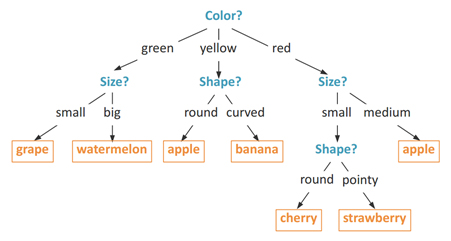
\includegraphics[width=0.5\textwidth]{figures/Structure.jpg}
  \caption{Example of a decision tree}
  \label{fig:ensemble learning}
\end{figure}

\subsection{Multiclass classification}

There are strategies for reducing a problem of multiclass classification to multiple binary classification problems. It can be categorized into One-versus-one (Build K (K-1) / 2 classifiers and make them vote) and One-versus-all (Build K classifiers and make them vote). To solve those problems, we have to use an algorithm that naturally handles multiple classes. It is the case of tree algorithms and Neural networks (that we will study in Chap. 10).\\

\subsection{Vocabulary Reminder}
Here is a short reminder of tree vocabulary:\\
\begin{figure}[h]
  \centering
  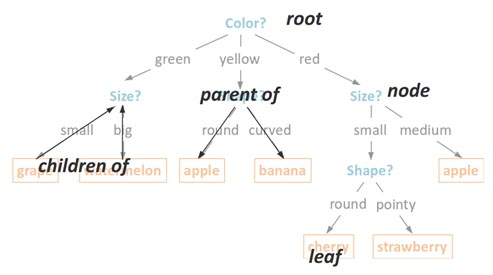
\includegraphics[width=0.5\textwidth]{figures/s1.jpg}
  \caption{Tree vocabulary}
  \label{fig:ensemble learning}
\end{figure}
\subsection{Partition of the feature space}

Classification and regression trees (CART) is the generic name for a recursive procedure to split a training set and organize it into a tree. The models are obtained by recursively partitioning
the training set into smaller and smaller subsets and fitting a simple prediction model within each partition. As a result, the partitioning can be represented graphically as a decision tree. During the CART procedure we will have to do several choices: 
\begin{itemize}
\item Binary or multi-way splits?
\item Which feature(s) to use at each node? i.e. how to split?
\item When to stop growing a tree?

\end{itemize}

\section{Binary-tree versus non binary-tree}

A binary tree is a tree data structure in which each node has at most two children, which are referred to as the left child and the right child. A tree with arbitrary branching factor can always be equivalently represented by a binary tree.  \\
The following binary tree is equivalent to the non-binary tree of Figure 1.

\begin{figure}[h]
  \centering
  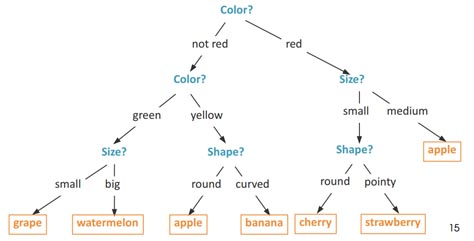
\includegraphics[width=0.5\textwidth]{figures/s2.jpg}
  \caption{Binary tree equivalent to Figure. 1}
  \label{fig:ensemble learning}
\end{figure}

\newpage
\section{How to grow a tree}

\subsection{Introduction}

We are only considering monothetic trees, that is to say trees with only one feature per node. In this conditions, the decision boundary is orthogonal to the axes. The splitting variable (j) and the splitting point (s) define 2 regions: \\
\begin{figure}[h]
  \centering
  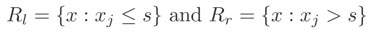
\includegraphics[width=0.5\textwidth]{figures/s3.jpg}
  \label{fig:ensemble learning}
\end{figure}


For a regression tree, we choose j and s to minimize SE (standard error):\\
\begin{figure}[h]
  \centering
  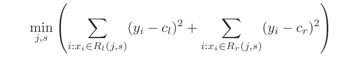
\includegraphics[width=0.5\textwidth]{figures/s4.jpg}
  \label{fig:ensemble learning}
\end{figure}


For a classification tree, we choose j and s to minimize impurity : \\
\begin{figure}[h]
  \centering
  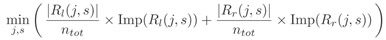
\includegraphics[width=0.5\textwidth]{figures/s5.jpg}
  \label{fig:ensemble learning}
\end{figure}

\subsection{Impurity}

Decision trees are grown by posing a series of questions about the feature of the items. In order to do so, we add question nodes incrementally, using labeled training examples to guide the choice of questions. Ideally, a single, simple question would perfectly split the training examples into their classes. If no question exists that gives such a perfect separation, we choose a question that separates the examples as cleanly as possible. \\

Several measures have been designed to evaluate the degree of inhomogeneity, or impurity, in a set of items. For decision trees, the most common measures are entropy, the Gini index and the classification error. Given a measure of impurity, we choose a question that minimizes the weighted average of the impurity of the resulting children nodes.

\subsection{Classification error}

The classification error corresponds to the minimum probability that a training point will be misclassied at node (s,j) and is defined by the following formula :
\[
\textrm{Imp}(R_m)= 1 - \textrm{max}_{  k}(\hat{p}_{mk})
\]
where \( \hat{p}_{mk} \) is the proportion of training instances from class k in \(R_m\). \\

The value of the classification error is always between 0 and 1. If all examples from one class belong to \(R_m\) then \( \textrm{Imp}(R_m)= 1 - \textrm{max}{(1)} = 0 \). If we have 2 balanced classes and instances are randomly split at (s, j), then \( \textrm{Imp}(R_m)= 1 - \textrm{max}{(
0.5, 0.5)} = 0.5 \)

\subsection{Entropy}

The concept of entropy comes from the information theory. Entropy is a measurement of information (or rather lack of information). We calculate the information gain by making a split. This measures how you reduce the uncertainty about the label. It is defined by the following formula:
\[
\textrm{Imp}(R_m)= -  \sum_{k}\hat{p}_{mk} \log_{2}(\hat{p}_{mk})
\]
where \( \hat{p}_{mk} \) is the proportion of training instances from class k in \(R_m\). \\

If all examples from one class belong to \(R_m\) then \( \textrm{Imp}(R_m) = 0 \). If we have 2 balanced classes and instances are randomly split at (s, j), then \( \textrm{Imp}(R_m)= - (\frac{1}{2}\log_{2}(\frac{1}{2})+ \frac{1}{2}\log_{2}(\frac{1}{2}))= 1 \)

\subsection{Gini Impurity}

Used by the CART (classification and regression tree) algorithm, Gini impurity is a measure of how often a randomly chosen element from the set would be incorrectly labeled if it was randomly labeled according to the distribution of labels in the subset. 

It is defined by the following formula:
\[
\textrm{Imp}(R_m)=  \sum_{k=1}^{K}\hat{p}_{mk}(1-\hat{p}_{mk})
\]
where \( \hat{p}_{mk} \) is the proportion of training instances from class k in \(R_m\). \\

If all examples from one class belong to \(R_m\) then \( \textrm{Imp}(R_m) = 0 \). If we have 2 balanced classes and instances are randomly split at (s, j), then \( \textrm{Imp}(R_m)= \frac{1}{2}\frac{1}{2}+ \frac{1}{2}\frac{1}{2}= \frac{1}{2} \) . \\

If we have two regions \( R_l \) and \( R_r \) then the impurity is defined by:
\[
\textrm{GI}(j,s)= \frac{\left | R_l(j,s) \right |}{n_{tot}}  \textrm{Imp}(R_l(j,s)) + \frac{\left | R_r(j,s) \right |}{n_{tot}}  \textrm{Imp}(R_r(j,s))
\]
Assuming that the split respects the overall distribution \( \forall k ,p_{mk}=\frac{\left | C_k \right |}{N} \) , then all regions are identically distributed and have Gini impurity:
\[
\textrm{GI}(R)= \sum_{k=1}^{K} \frac{\left | C_k \right |}{N}  (1-\frac{\left | C_k \right |}{N} ) = 1 - \sum_{k=1}^{K} (\frac{\left | C_k \right |}{N})^{2} \]

For a K-way split  \(\textrm{GI}(j,s)= \sum_{l=1}^{K} \frac{1}{K} \textrm{GI}(R) = \textrm{GI}(R)\) and in particular if \(\left | C_k \right | = \frac{N}{K} \) then \(\textrm{GI}= 1 - \frac{1}{K} \). If the split is perfect then all regions have a proportion of 1 of one class and of 0 of
the other, and hence have Gini impurity \(\textrm{GI}(R)=0 \).


\subsection{When to stop growing a tree?}

If a tree is too large it might overfit while a small tree might underfit. Therefore we have to establish a strategy in order to decide when to stop growing a tree.
There are two main strategies:
\begin{itemize}
\item we can either grow the tree until a minimum node size (number of training points in the region) is reached
\item or we can prune the tree using cost-complexity pruning
\end{itemize}

\subsection*{Cost-complexity pruning}

In a similar way to what we did with regularisation we define the cost complexity with the following formula which includes a complexity penalty :
\[
C_\alpha (Tree)=  \sum_{m=1}^{\# Tree} N_m Q_m(Tree) + \alpha (\# Tree)
\]
where:
\begin{itemize}
\item \#Tree is the number of regions in our pruned tree
\item \(N_m\) is the number of training instances in \(R_m\)
\item \(Q_m\) is the error on \(R_m\)
\item \(\alpha \) is a coefficient which defines the balance between model complexity and goodness of fit
\end{itemize}

The goal is to find a subtree which will minimise the cost-complexity.
The more leaf nodes that the tree contains the higher complexity of the tree because we have more flexibility in partitioning the space into smaller pieces, and therefore more possibilities for fitting the training data. There is also the issue of how much importance to put on the size of the tree. The complexity parameter \(\alpha \) adjusts that.

\section{Advantages and drawbacks of trees}

\begin{tabular}{|c|c|}
  \hline
  Advantages & Drawbacks  \\
  \hline
  Easy to explain & Bad predictive accuracy in general  \\
  Mirror human-decision making & \\
  Displayed graphically and easily interpreted & \\
  Can easily handle quatitative variables & \\
  Naturally handle multiclass problems & \\
  \hline
  
\end{tabular}\\

In order to improve the predictive accuracy we will use forests. 

\newpage
\section{Forest}


\paragraph{Ensemble learning.}The idea is that aggregating many weak learners can substantially increase their performance, because trees have weak predictive power in general. This method is called ensemble learning and uses the principle of wisdom of crowds, that by combining multiple individual classifiers, we can average out their uncorrelated errors. This is what we can observe with the example below, by combining many 'staircase' boundaries, we finally obtain a diagonal separation. \\

\begin{figure}[h]
  \centering
  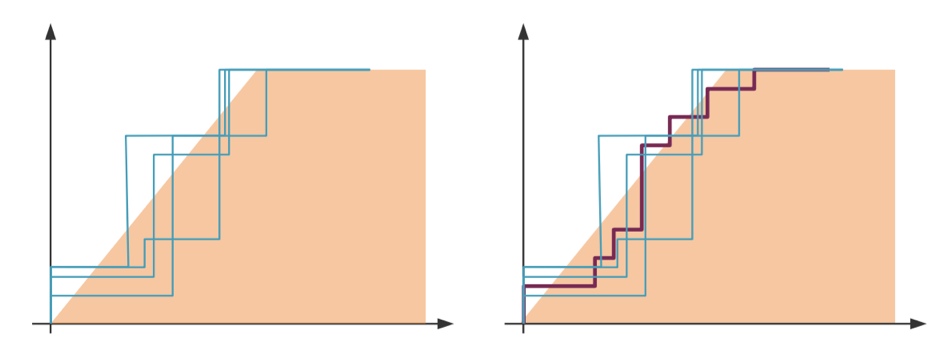
\includegraphics[width=0.5\textwidth]{figures/Staircase.png}
  \caption{Principle of ensemble learning}
  \label{fig:ensemble learning}
\end{figure}

\subsection{Building ensembles}

To build ensembles, we have to:

\begin{itemize}
\item \textbf{subsample the training data} : by either bagging the data, picking multiple times the same point, or boosting which is resampling based on performance.

\item Use \textbf{different features} (with multiple input representations, we will also learn how to select features in the chapter 11).


\item Use different \textbf{parameters} of the learning algorithm.\\

\end{itemize}

When we combine weak learners : 

\begin{itemize}
\item if it is a non-trainable combination: it should be done by \textbf{voting} (classification) or \textbf{averaging} (regressing).


\item if it is a trainable combination: we use \textbf{weighted averaging} based on performance on a validation set or \textbf{meta-learner} with which the outputs of the individual learners are features for another learning algorithm. 

\end{itemize}

\subsection{Bagging trees}

The principle is to bootstrap the training data (take repeated samples) and build one predictor from each of these samples. The final prediction is the \textbf{average} of the samples when considering a \textbf{regression} problem and a \textbf{majority vote} for a \textbf{classification} problem.


\subsection{Random forest}

The idea in random forests is to improve the variance reduction of bagging by reducing the correlation between the trees, without increasing the variance too much. This is achieved in the tree-growing process through random selection of the input variables: before each split, select q (out of p) input variables at random as candidates for splitting. We typically choose q = $\sqrt[]{p}$ .
This method has very good predictive power in practice!

\section{Summary}

Decision trees are easy to interpret.\\
Decisions trees elegantly deal with :
\begin{itemize}
\item Quantitative variables
\item Multiple classes
\item Multimodal distributions
\end{itemize}
Decision trees have limited predictive power, but this can be addressed thanks to ensemble methods:
\begin{itemize}
\item Bagging 
\item Random forests 
 \end{itemize}
\end{document}